\subsection{DNR with SVM}

The first implementation trains a Support Vector Machine model to perform classification of BIO tag for each word as a means of Drug Name Recognition. All code is based on Python 3 and Scikit-learn and uses modules for interacting with Freeling, perform the lookup of words on a DrugBank lookup and the like. The model used is a linear support vector machine, which will use the DictVectorizer library from Scikit-learn to transform the feature vector into a suitable format consisting of only binary variables. 

\textbf{Features}

The complete set of features prepared for this model are the following:
\begin{table}[H]
\centering
\begin{tabular}{lcl}
\multicolumn{3}{l}{DNR features}                                                                                                               \\ \hline
$f_{1}$ & Word feature             &                                                                                                                               \\
\rowcolor[HTML]{DAE8FC} 
$f_{2}$ & Part-Of-Speech           &                                                                                                                               \\
$f_{3}$ & Lemmatization           &                                                                                                                               \\
\rowcolor[HTML]{DAE8FC} 
$f_{4}$ & Orthographic - basic features     & \begin{tabular}[c]{@{}l@{}}5 classes: \\ all-capitalized, is-titlecase,all-digits,\\ alphanumeric, hyphen or not\end{tabular} \\
$f_{5}$ & Orthographic - affix features           & Prefixes and suffixes of the length 3,4,5                                                                                     \\
\rowcolor[HTML]{DAE8FC} 
$f_{6}$ & Orthographic - Word shape features      & \begin{tabular}[c]{@{}l@{}}Generalized word class: Xxxxx00xxOxx \\ Brief word class: Xx0xOx\end{tabular}                      \\

$f_{7}$ & Dictionary features      & Lookup on Drugbank                                                                                            \\
\rowcolor[HTML]{DAE8FC} 
$f_{8}$ & Chunk feature            &    NLTK noun phrase chunking tag                                                                                                                         \\
$f_{9}$ & Word Embeddings features & Word2Vec and classification                                                                                                  
\end{tabular}
\caption{DNR features}
\label{table:DNRfeatures}
\end{table}
The drug name lookup is performed on the Drugbank dictionary xml file, parsed in memory as a Python dictionary that allows to query for existence of the word as a key. The chunker feature is obtained from NLTK named entity chunker, returning chunk and chunkGroup for each word in the sentence. 
The Word2Vec feature was obtained from a pretrained 200 window length Word2Vec model from PubMed, where the coordinates of each word where added to the feature vector.
The BIO tag class type is obtained by processing the indications of char offsets for entities in each sentence. In order to avoid any conflict with the Freeling analyzers, the BIO tag matching is done after tokenization and pos taging modules of Freeling are executed. All the orthographic are obtained from the words and their basic lemma and POS-tag features in an adjustable window from 0 to 5. 

\textbf{Feature vector}

The SVM model is trained on a word features basis. This includes all the possible features of a word and the words in a context window of 0 to 5.  This means that the model to be trained will receive a feature matrix consisting of a feature vector for each word of each sentence in the training data set. The structure of the feature vector for each word is shown in the figure \ref{dnrsvm}.

\begin{figure}[H]
\centering
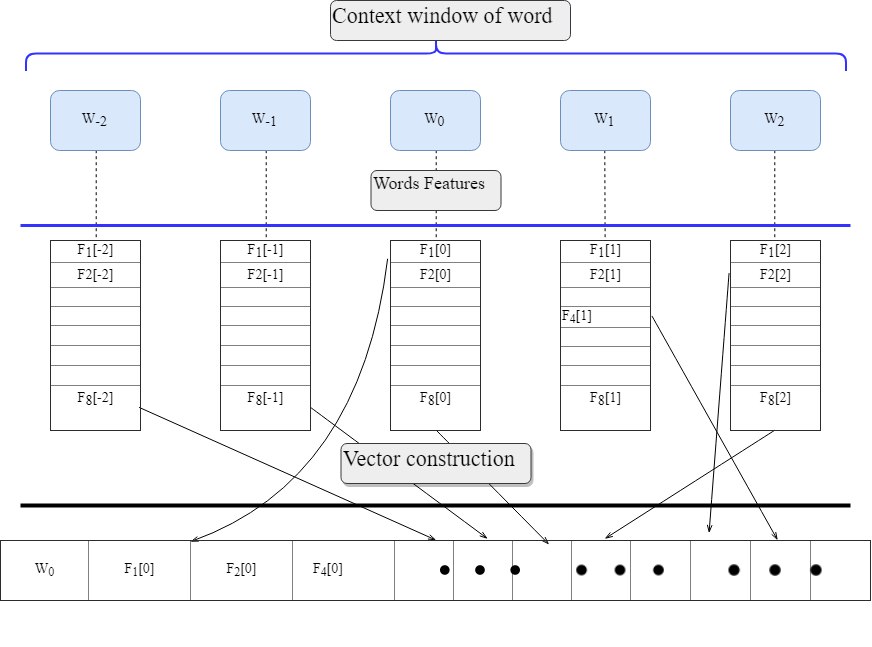
\includegraphics[scale=0.3]{VectorConstruction.png}\caption{DNR-SVM feature vector}\label{dnrsvm}
\end{figure}




